\documentclass[10pt,twocolumn,letterpaper]{article}


\usepackage{cvpr}
\usepackage{times}
\usepackage{epsfig}
\usepackage{graphicx}
\usepackage{amsmath}
\usepackage{amssymb}
\usepackage{hyperref}
\usepackage{listings}
\usepackage{url}
\usepackage{xcolor}
\usepackage{float}
\usepackage{booktabs}
\usepackage{cleveref}
\usepackage[numbers]{natbib}
\usepackage{subcaption}
\usepackage{tabularx}
% Include other packages here, before hyperref.

\definecolor{codegreen}{rgb}{0,0.6,0}
\definecolor{codegray}{rgb}{0.5,0.5,0.5}
\definecolor{codepurple}{rgb}{0.58,0,0.82}
\definecolor{backcolour}{rgb}{0.95,0.95,0.92}



\lstdefinestyle{cppstyle}{
    backgroundcolor=\color{backcolour},   
    commentstyle=\color{codegreen},
    keywordstyle=\color{magenta},
    numberstyle=\tiny\color{codegray},
    stringstyle=\color{codepurple},
    basicstyle=\ttfamily\footnotesize,
    breakatwhitespace=false,         
    breaklines=true,                 
    captionpos=b,                    
    keepspaces=true,                 
    numbers=left,                    
    numbersep=5pt,                  
    showspaces=false,                
    showstringspaces=false,
    showtabs=false,                  
    tabsize=2,
    language=C++,
    morekeywords={pragma, omp, parallel, for, simd, schedule, static}
}


\setcitestyle{square}
\lstset{style=cppstyle}
% If you comment hyperref and then uncomment it, you should delete
% egpaper.aux before re-running latex.  (Or just hit 'q' on the first latex
% run, let it finish, and you should be clear).
%\usepackage[pagebackref=true,breaklinks=true,letterpaper=true,colorlinks,bookmarks=false]{hyperref}

\cvprfinalcopy % *** Uncomment this line for the final submission

\def\cvprPaperID{****} % *** Enter the CVPR Paper ID here
\def\httilde{\mbox{\tt\raisebox{-.5ex}{\symbol{126}}}}

% Pages are numbered in submission mode, and unnumbered in camera-ready
\if4cvprfinal\pagestyle{empty}\fi
\begin{document}
%%%%%%%%% TITLE
\title{MeanShift: Analysis of speedup achieved through parallel programming on CPU}

\author{Emanuele nencioni\\
E-mail address\\
{\tt\small emanuele.nencioni@edu.unifi.it}
% For a paper whose authors are all at the same institution,
% omit the following lines up until the closing ``}''.
% Additional authors and addresses can be added with ``\and'',
% just like the second author.
% To save space, use either the email address or home page, not both
}

\maketitle
\thispagestyle{empty}

%%%%%%%%% ABSTRACT
\begin{abstract}
   This report presents the implementation and performance analysis of different versions of the Mean Shift clustering algorithm\cite{first_mean_shift}, applied to image segmentation. This is a robust non-parametric technique; however, its computational complexity $\mathcal O(N^2)$ presents a significant bottleneck for sequential execution on high-resolution data. In this report, the algorithm was optimized and parallelized using the OpenMP framework. Through an evaluation from a series of experiments (focused on execution time, speedup, and efficiency) The results show that parallel implementation effectively reduces processing time. Furthermore, the report provides a detailed analysis of the performance impact of thread scheduling and memory access patterns, validating the effectiveness of the chosen parallelization strategies.
\end{abstract}

%%%%%%%%% BODY TEXT
\section{Introduction}
Mean Shift\cite{first_mean_shift} is a non-parametric clustering technique used for "mode-seeking" in a feature space (\Cref{fig:mshift}). Unlike algorithms such as K-Means\cite{macqueen1967multivariate}, Mean Shift does not require an \textit{a priori} specification of the number of clusters.  Instead, it discovers the underlying structure of the data by iteratively shifting each point toward the local density gradient.

In the context of image segmentation, the algorithm maps each pixel into a five-dimensional (5D) joint spatial-range domain:
$$\mathbf{x} = [r, g, b, x, y]^\top$$ 
where $(r, g, b)$ represents the color components and $(x, y)$ denotes the spatial coordinates.  This  introduces a significant computational burden, but this high-dimensional mapping allows for sophisticated segmentation that respects both color similarity and spatial proximity.

\subsection{Kernel Density Estimation and Mode Seeking}
In the joint spatial-color domain, the density at a point $\pmb x$ is estimated using a kernel $K$ with bandwidth $h$. The Mean Shift algorithm seeks the modes of this density function by following the gradient. Mathematically, for each pixel i, we compute the Mean Shift vector $m(\pmb x_i)$:

$$m(\pmb x_i)=\frac{\sum_{j=1}^n\pmb x_jK\bigg(\frac{\|\pmb x_i-\pmb x_j\|^2}{h^2}\bigg)}{\sum_{j=1}^nK\bigg(\frac{\|\pmb x_i-\pmb x_j\|^2}{h^2}\bigg)}-\pmb x_i$$

This vector $m(\pmb x_i)$ always points to the direction of the maximum increase in density. The algorithm iteratively updates $\pmb x_i\gets \pmb x_i+m(\pmb x_i)$ until the magnitude of the shift  vector $\|m(\pmb x_i)\|$ falls below a threshold $\epsilon$.

Within a Brute-force approach, each of the $N$ pixels must query all the other $N$ in the image to calculate the weighted mean, resulting in a computational complexity of $\mathcal O(N^2)$. While literature often distinguishes between spatial ($h_s$) and range ($h_r$) bandwidths  to fine-tune the filtering effect (Comaniciu et al. 2002 \cite{double_bandwidth}), this implementation utilizes a unified bandwidth h. This choice preserves the fundamental interaction logic and the $\mathcal O(N^2)$ complexity while maintaining the project's primary focus on  optimization and parallel efficiency rather than the heuristic tuning of clustering output. 

\begin{figure}
    \centering
    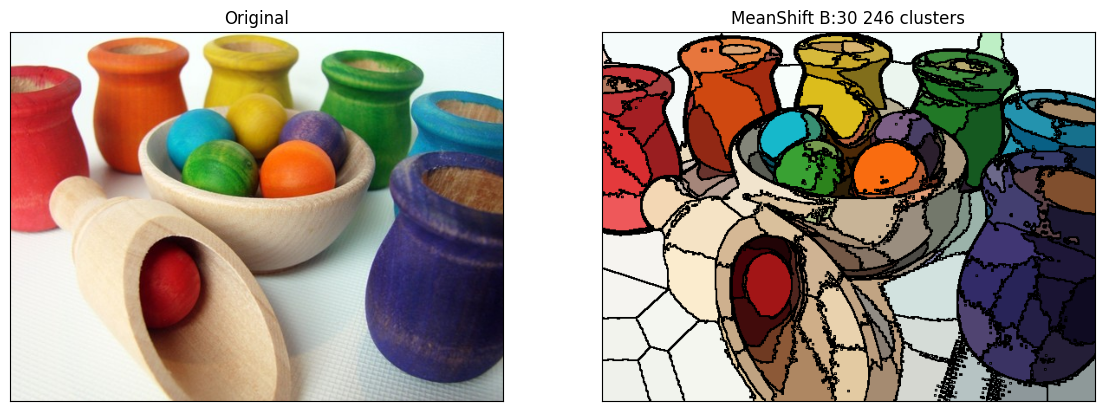
\includegraphics[width=1\linewidth]{images/mshift5.png}
    \caption{left: Original image, right: mean shift clustering with bandwith of 30, black borderds.}
    \label{fig:mshift}
\end{figure}

\section{language and frameworks}
The implementation is developed in C++, selected for its ability to provide explicit control over memory alignment and hardware-level optimizations required for high-performance computing. The software architecture leverages SIMD Vectorization since C++ enables the use of compiler intrinsics and auto-vectorization (e.g., AVX2/AVX-512) to exploit Instruction-Level Parallelism. In this way, the 5D distance calculations can be processed as vector operations, significantly increasing the floating-point throughput per clock cycle. Parallelism is achieved through the OpenMP framework, which is uniquely suited to Mean Shift\cite{first_mean_shift} due to its embarrassingly parallel nature.  Since the mode-seeking trajectory of each pixel is independent, the workload allows for a data parallel decomposition. Lastly, OpenCV is utilized as a post-processing tool for data visualization and qualitative analysis of the segmentation boundaries.

\section{Methodology}\label{sec:method}
This current project will see different implementations designed specifically for three-channel RGB images, focusing on the standard 5D joint spatial-range domain. For a proper performance analysis, the basic form of the algorithm was first implemented using brute-force approach with sequential computation ( $\mathcal O(N^2)$). Then it follows a progressive optimization path to address specific bottlenecks:
\begin{enumerate}
\item \textbf{Refined Sequential Baseline (\texttt{seq})}, An optimized version designed to remove redundant ALU overhead by pre-computing spatial coordinates.
\item \textbf{Structure of Arrays (\texttt{soa})}, A memory-reorganization approach aimed at improving data locality and helping SIMD auto-vectorization.
\item \textbf{Parallel AoS (\texttt{omp})}, A multi-threaded implementation utilizing OpenMP on the interleaved memory layout.
\item \textbf{Parallel SoA (\texttt{omp\_soa})}, A hybrid approach combining the benefits of the SoA layout with shared-memory parallelization.
\end{enumerate}
All the code of each implementation is available in the Appendix \ref{sec:appendix}.


\subsection{Baseline implementation}
First, the algorithm (see appendix \ref{subsec:baseline}) computes the mean shift vector of the neighbor centered on the current pixel, with a bandwidth $h$. The result is a vector directed towards the highest increase in the gradient of density function. Using a uniform kernel, this vector can be represented as a vector difference of the arithmetic average (or centroid) of all points in a 5D window  of a particular size $h$ minus the current point's location.  Then, each pixel's state is shifted according according to its mean shift vector to the local centroid. 

From a structural perspective, the baseline source code reveals a three-level nested loop hierarchy that dictates the algorithm's execution flow and computational complexity. The \textbf{Temporal Loop} (outermost) manages the iterative refinement process; it will execute the entire mean shift pipeline until convergence or a max number of iterations is reached. Within this, the \textbf{Spatial loop} iterates through the $N$ pixels of the images, treating each one as an independent agent seeking a local density mode. Finally, the \textbf{Neighbor loop} queries all N pixels in the image to compute the mean-shift vector and the kernel calculation. The interaction between these two inner loops generates the quadratic $\mathcal O(N^2)$.

This method utilizes an interleaved memory layout, which can be defined as a \textit{logical} Array of Structures (AoS) (\cref{code:aos_impl}). Although the data are stored in a flat \texttt{std::vector<float>} rather than a formal C++ \texttt{struct}, the memory footprint is identical to an interleaved layout where all components of a single data element (the RGB channels) are stored contiguously ($[R_0,G_0,B_0,R_1,G_1,B_1,…]$). This often requires de-interleaving for efficient SIMD processing. In this case, this contiguous grouping provides high spatial locality for single-pixel operations, but introduces a stride-3 access pattern for individual color channels. This makes the loop difficult to auto-vectorize.

\begin{lstlisting}[language=C++, caption={baseline Image implementation}, label={code:aos_impl}]
struct STBImage {
    int width{0}, height{0}, channels{0};
    uint8_t* rgb_image{nullptr};
    std::string filename{};
    ~STBImage();
    bool loadImage(const std::string& name);
    void saveImage(const std::string& newName) const;
};
\end{lstlisting}

\subsection{\textit{seq} implementation}\label{subsec:seq}
In the initial baseline design, the spatial coordinates (x,y) of each pixel were dynamically derived  from the linear index j using the image width (\cref{code:aos_spatial}). While this approach minimizes the memory footprint by avoiding the storage of redundant spatial data, it shifts the primary bottleneck to the CPU's execution units. Integer division (\texttt{/}) and modulo (\texttt{\%}) are among the highest-latency scalar instructions on modern x86 architectures. Performing these operations $N^2$ times per iteration  can causes the inner loop to become heavily \textbf{compute-bound}. To prioritize execution efficiency, in this new implementation,  spatial coordinates are pre-computed and stored within the feature vector(\cref{code:aos_spatial_mem}). This expansion of the 'pixel' data structure effectively trades memory capacity for a significant reduction in clock cycles per iteration, transforming the algorithm into a more efficient memory-bound process. As a result, the initial \texttt{stb\_image} buffer is replaced by a tailored data layout.

Another improvement involved \textbf{memory hoisting}, implemented by moving the auxiliary buffer allocations outside the \textbf{temporal loop}. This can reduces the overhead of the memory manager by avoiding O(iter) system calls and heap allocations. This was maintained across the subsequent implementations described in this section.

\begin{lstlisting}[language=C++, caption={seq spatial save into pixel struct}, label={code:aos_spatial_mem}]
struct Pixel {
    float r, g   , b;
    float x, y; 
};
\end{lstlisting}

\subsection{SoA implementation}\label{subsec: SoA}
In the previously described AoS layout, each pixel is represented by a contiguous block of five floating-point values. Although this ensures locality for individual pixel updates, it introduces a stride-5 access pattern when the algorithm evaluates a specific dimension across the dataset.  This non-contiguous access can be suboptimal as it complicates the "gathering" of data into vector registers.

To mitigate these limitations, the Structure of Arrays (SoA) implementation reorganizes the memory layout by decomposing the feature vectors into five independent contiguous arrays $(V_R,V_G,V_B,V_x,V_y)$, each of size N ( \cref{code:soa_impl_with_neigh_acc}). This architectural shift provides two primary advantages:
\begin{enumerate}
\item \textbf{SIMD Vectorization}, the SoA layout is inherently "SIMD-friendly." Because values of the same dimension are stored contiguously, the compiler can leverage SIMD extensions,  to load and process eight pixels simultaneously in a single 256-bit register. This can eliminate the need for expensive shuffle or de-interleaving instructions required by the AoS layout.
\item \textbf{Unit-Stride Memory Access}, by ensuring that data are accessed with a stride of one, the implementation can maximize cache-line utilization. When the processor fetches a cache line, it retrieves multiple relevant values for a single dimension, reducing the total number of memory requests and improving overall throughput.
\end{enumerate}
The transition from the interleaved \texttt{stb\_image} format to this SoA representation is handled during the initialization phase. 

\subsection{\textit{omp} implementation}
In this other implementation an attempt to parallelize the seq implementation was made trying to achieve even more performance boost. The analysis started from the identification of the optimal level of parallelism on each loop: the \textbf{temporal loop}, the external one, isnt paralelizable due to temporal dependencies (the new iteration depend on the previous one), the \textbf{neighbor loop} (innermost) would trigger a "fork-join" operation, for example, given an image with a standard resolution, this would results in hundreds of thousands of thread synchronization per second, leading to massive overhead that would dwarf the actual computation. The \textbf{Spatial loop} is the answer, Each thread is assigned to a contiguous block of pixels to process independently.

\subsubsection{Reduction and thread safety}
The algorithm must track the maximum shift magnitude across all pixels in order to determine convergence. In the sequential environment this is straightforward (\lstinline[language=C++]{if(change > max_change) max_change = change;}) but in a parallel environment there are multiple threads attempting to update `max\_change` generating a \textbf{race condition}. To resolve this, the implementation uses the OpenMP \textbf{reduction} clause (\cref{code:omp_focus_loop}).  This allows each thread to maintain a locale and private maximum within its own registers or L1 cache. Only upon termination of the parallel region, OpenMP performs a single thread-safe comparison of these local values (typically via a tree-based reduction) to update the global variable. 

\begin{lstlisting}[language=C++, caption={Parallel decomposition of the spatial loop utilizing OpenMP max-reduction for thread-safe convergence tracking.}, label={code:omp_focus_loop}]
#pragma omp parallel for reduction(max: max_change)
for(int i = 0; i < n_pixels; ++i) {
    // ... computation ...
    if(change > max_change) max_change = change;
}
\end{lstlisting}
\subsubsection{Memory hoisting and Jacobi semantics}
While memory hoisting was introduced in the seq implementation, it becomes fundamental to the performance of this one. In a multi-threaded environment, leaving the auxiliary buffer outside avoids \textbf{thread starvation} where worker threads can remain idle while the master thread performs the sequential task of allocating a new vector. In this way, the implementation reduces the serial overhead between successive iterations, maximizing core utilization.


The use of separate "current" and "next"(\cref{code:mem_omp}) buffers enforces \textbf{Jacobi semantics}, which provides the mathematical foundation for thread safety. This also allows the \textbf{spatial loop} to strictly adhere to \textbf{Bersnstein's conditions} for parallel executions:
\begin{itemize}
    \item \textbf{flow and anti-dependence} are avoided by ensuring that threads only read from the \textit{current} and only write on the \textit{next} buffers,
    \item \textbf{output dependence} is deleted since each thread is assigned a unique pixel index $i$ in the output array, removing the risk of multiple threads attempt to write to the same memory address.
\end{itemize}
 Consequently, the algorithm removes \textbf{READ-AFTER-WRITE (RAW)} hazards without the need for costly synchronization primitives, such as \textit{atomic} or \textit{critical} sections. This  ensures that the parallel version of the means shift algorithm \cite{first_mean_shift} is bit-wise identical to the sequential version.


\begin{lstlisting}[language=C++, caption={Structural implementation of buffer hoisting and Jacobi double-buffering.},label={code:mem_omp}, basicstyle=\small\ttfamily]
// Memory Hoisting: Buffer allocated once outside the temporal loop
std::vector<Pixel> next(n_pixels); 

for(; iter < max_iter; ++iter) {
    #pragma omp parallel for schedule(static)
    for(int i = 0; i < n_pixels; ++i) {
        // ... compute new_pixel based on "current" snapshot ...
        next[i] = new_pixel; // Write to auxiliary buffer
    }

    // Jacobi Semantics: O(1) pointer swap to prepare for next iteration
    current.swap(next); 
}
\end{lstlisting}

\subsection{\textit{omp\_soa} implementation}
The final refinement of the algorithm integrates the Structure of Arrays (SoA) memory layout with OpenMP multithreading. This version represents the most optimized form of the Mean Shift implementation, as it addresses both computational throughput and memory bandwidth efficiency.

\subsubsection{Data locality and thread efficiency}
In the standard OpenMP implementation using a Point-of-Pixels (AoS) layout, each thread must load interleaved R, G, and B values into registers. By switching to SoA, each thread now accesses contiguous blocks of memory for each color channel. This enables significantly improves the cache hit rate during the parallel spatial loop.

The spatial locality is maximized due to the separation of the feature space components into large, independent arrays. This reduces memory bandwidth bottlenecks and keeps the execution units saturated.

As previously established, the SoA layout is a prerequisite for efficient SIMD operations; consequently, this contiguous memory access enables each individual core to directly leverage vector instructions.

\begin{lstlisting}[language=C++, caption={baseline spatial indexing}, label={code:aos_spatial}]
float xj = static_cast<float>(j % width);
float yj = static_cast<float>(j / width);
\end{lstlisting}
\subsection{CUDA implementation}

\section{Testing Environment and Methodology}
The experiments were conducted on a workstation featuring the AMD Ryzen 9 9900X processor, based on the Zen 5 architecture. This CPU provides 12 physical cores (24 logical threads via SMT) with a 64 MiB shared L3 cache. In \cref{tab:components} are summarized more software and hardware specifications. 32 GB of RAM and a Nvidia GeForce GTX 1060 with 6GB of VRAM. The experimental evaluation was conducted on a workstation featuring an AMD Ryzen 9 9900X processor. This CPU integrates 12 physical cores with 24 logical threads via Simultaneous Multithreading (SMT) and features a 64 MiB shared L3 cache. The system is also equipped with 32 GB of main memory and an NVIDIA GeForce GTX 1060 GPU with 6 GB of VRAM. A comprehensive summary of the hardware and software environment is provided in \cref{tab:components}.

\begin{table}[]
    \centering
    \begin{tabular}{|c|c|}
    \hline
           Component &  Specification \\
           \hline\hline
         OS & Arch Linux (kernel 6.19.14) \\
         \hline
         Compiler & GCC 16.11 (C++17 standard) \\
         \hline
         Optimization Flags & \texttt{-O3 -march=native} \\
         \hline
         Parallel runtime & OpenMP (bundled with GCC) \\
         \hline
         Memory & 32 GiB DDR5 RAM \\
    \hline
    \end{tabular}
    \caption{Benchmark workstation spec's summary}
    \label{tab:components}
\end{table}

\subsubsection{Clock Selection and Benchmarking Methodology}
For all performance measurements, \texttt{std::chrono::steady\_clock} was used instead of \texttt{std::chrono::high\_resolution\_clock}. While the latter suggests higher precision, the C++ standard does not guaranty its steadiness; on some implementations, it may alias the system wall-clock, making it susceptible to timing discontinuities (e.g. NTP adjustments). In contrast, \texttt{steady\_clock} is guaranteed to be monotonic, ensuring that elapsed time measurements remain consistent and reproducible across different execution environments. On the Ryzen 9900X test platform, this clock provides nanosecond resolution, which is more than sufficient for capturing the micro-scale performance in the different  implementations.

\subsubsection{Dataset and benchmark setup}
The testing methodology was rigorously designed  to evaluate the scalability and architectural efficiency of the various Mean Shift\cite{first_mean_shift} implementations. This isolates computational workload (pixel count) from convergence complexity (image texture and gradients)

\subsubsection{Dataset}
Initial testing utilized synthetic inputs, such as solid-color and flat-gradient images (e.g., \texttt{solid\_100.png} or \texttt{red400.png}). However, these were discarded because they typically converge in a single iteration, failing to provide a realistic workload for correct profiling.

The standard Berkeley Segmentation Dataset (BSD500) was utilized to ensure that the algorithm operates in a regime requiring multiple iterations, essential for accurate speedup and parallel efficiency profiling. These natural photographs contain smooth gradients, textured regions, and overlapping color distributions that provide a realistic stress test for the Mean Shift\cite{first_mean_shift}. In particular, the benchmark employs a $5 \times 5$ cross-validation grid yielding 25 test configurations. Five distinct source images, ranging from "low" to "very high" complexity, are evaluated across five geometric resolution tiers (ranging from 6,700 to 68,480 pixels). By running all 5 source images at each of the 5 resolution tiers, execution times can be averaged across sources. This yields a tier-representative mean that isolates the scaling impact of pixel count without being biased by the convergence behavior of any single image.

\subsubsection{Benchmarking Parameters}
Parallel scaling analysis requires speedup $(S = T_1 / T_p)$ to be defined over a strictly fixed amount of work. Consequently, the benchmark deliberately caps the convergence loop at a maximum of 5 iterations (\texttt{MAX\_ITER = 5}). This configuration explicitly isolates the per-iteration cost of the algorithm's inner loop rather than measuring stochastic total convergence time. Furthermore, the benchmark stresses the micro-architecture by varying the spatial-color bandwidth parameter ($h \in \{20, 50, 100\}$): $h = 20$ produces tight clusters and short ranges, demanding many iterations and yielding high compute intensity per iteration; $h = 100$ instead, create large neighborhoods, forcing broad spatial scans that test the system's transition toward memory-bandwidth saturation.


Additionally, for every single test configuration (image, algorithm, and thread count), an initial unmeasured run is executed to warm up the hardware state. This preliminary execution ensures that the L1/L2 data and instruction caches are populated, branch predictors are primed, and operating system demand-paging overheads are resolved. Consequently, the subsequent timed iterations strictly measure the steady-state algorithmic performance, preventing initialization latency from skewing the microarchitectural profiling.
\section{Result and discussion}
This section presents the performance evaluation of the four Mean Shift implementations. By sweeping across a multi-dimensional benchmark matrix, we analyze how the architectural optimizations discussed in \cref{sec:method} translate into real-world speedups on modern consumer hardware. TALK HERE ABOUT perf.

\subsubsection{The kernel problem}
At first, a swappable kernel was implemented to actually test each one within the benchmark. This outlined a problem: SIMD operations can only be utilized when there is no variability in this function. Since the kernel is choosen at runtime, all the benchmark resulted in worst cases possible using SoA. So since the project doesn't have to focus on the kernel quality of the segmentation results, It was decided to hard code the flat kernel. Graphs of this problem can be found in the Appendix (
%%% Parlare di cosa si può cambiare: bandwith, kernel... img_size, tante variabili
%%%
\subsection{SoA vs seq vs baseline} \label{subsec:soa_seq_base}
The empirical results corroborate the architectural design choices detailed in \cref{sec:method}. As shown in \cref{fig:aos_soa}, the performance hierarchy remains consistent across all resolution tiers, with the SoA variant providing the most significant reduction in execution latency. The 2.8× time reduction observed for the SoA variant over the Baseline validates the transition to unit-stride memory access discussed in \cref{subsec: SoA}. While the seq(AoS) version reduces ALU pressure by pre-computing coordinates, the SoA version successfully mitigates the "cache pollution" inherent in interleaved data structures, allowing the hardware to maximize throughput.  An important finding is the near-identical performance in varying bandwidth parameters ($h$). Despite the theoretical increase in the spatial search range when $h=100$, the execution time does not scale linearly with the search volume. This suggests that the bottleneck on the Ryzen 9900X is not the memory bus bandwidth, but rather the L1/L2 cache hit latency and the instruction retirement rate of the inner loop's comparison logic. Lastly, the "Baseline" implementation shows a growing latency increase at higher resolutions with respect to seq. This confirms that the overhead of on-the-fly coordinate recomputation (\cref{code:aos_spatial}) dominates the execution time as $N$ grows, while the optimized versions (\cref{subsec:seq} \& \cref{subsec: SoA}) maintain a more favorable scaling curve by shifting the workload to vectorizable floating-point operations. 
\subsubsection{Some deeper analysis} \label{subsubsec:profiling}
Something strange happened in the data, cause looking at \cref{tab:performance_comparison}, the results are counter-intuitive. the SoA implementation result with an Higher L1 miss rate and lower IPC than AoS and baseline too. But if we actually go and watch the raw data, we can clearly see that the Absolute L1 miss count is Identical to all 3 implementations. The rate is actually missleading cause the SoA implementation reduce instructions, load operations and cycles by 3x. So the miss rate ( misses / loads) goes up. This is a confirm that the SIMD instructions are actually used and are benificial in the SoA implementation.

As shown in \cref{tab:performance_comparison}, the per-instruction metrics produce a counter-intuitive picture: the \texttt{soa}implementation exhibits a higher L1\,D-cache miss rate and a lower IPC than both \texttt{seq} and \texttt{baseline}. Taken in isolation, these figures would suggest that the SoA memory layout is \emph{detrimental} to cache behavior. However, inspecting the raw counter values reveals that this interpretation is incorrect. As \cref{fig:profile_l1_miss_count} shows, the \emph{absolute} number
of L1\,D-cache misses is virtually identical across all three implementations $\approx 294\,\text{M}$). The elevated miss \emph{rate} is therefore an arithmetic artifact rather than a sign of additional cache pressure. The root cause is visible in \cref{fig:profile_l1_loads,fig:profile_instructions}:
the \texttt{soa} implementation issues approximately $3\times$ fewer load operations
and retires $3\times$ fewer instructions than \texttt{seq}. Since the L1 miss rate
is defined as $\text{misses} / \text{loads}$, a threefold reduction in the
denominator inflates the rate even when the numerator stays constant. The same
effect depresses the IPC figure, because IPC is similarly normalized per retired
instruction rather than per unit of useful work.
This behaviour is consistent with the compiler auto-vectorising the SoA inner
loop using SIMD instructions (AVX2 on the test machine), each of which processes
multiple pixels simultaneously and therefore counts as a single load and a single
retired instruction in the hardware counters. The direct consequence is visible in
\cref{fig:profile_cycles}: \texttt{soa} completes in approximately $3\times$ fewer
CPU cycles than \texttt{seq}, confirming that the SIMD widening translates
directly into a proportional reduction in execution time.
In summary, the per-instruction metrics (IPC, L1 miss rate) are misleading when
SIMD is involved, because their denominators collapse with instruction count. The
correct metrics to compare implementations under vectorisation are the
\emph{absolute} counters --- total cycles, total instructions, and total stall
slots --- all of which show \texttt{soa} as the clear winner.
\begin{table}[htbp]
\centering
\caption{Sequential implementations profiling comparison}
\label{tab:performance_comparison}
\begin{tabular}{l c c c}
\toprule
\textbf{Metric} & \textbf{Baseline} & \textbf{seq (AoS)} & \textbf{soa (SoA)} \\
\midrule
IPC                  & 2.80   & \textbf{3.03}   & 2.36   \\
L1 miss rate         & 9.0\%  & 12.2\% & \textbf{30.8\%} \\
LLC miss rate        & 0.48\% & \textbf{0.50\%} & 0.46\% \\
Backend stalls/cycle & 4.98   & 4.71   & \textbf{5.06}   \\
\bottomrule
\end{tabular}
\end{table}

\begin{figure*}    
\begin{center}
    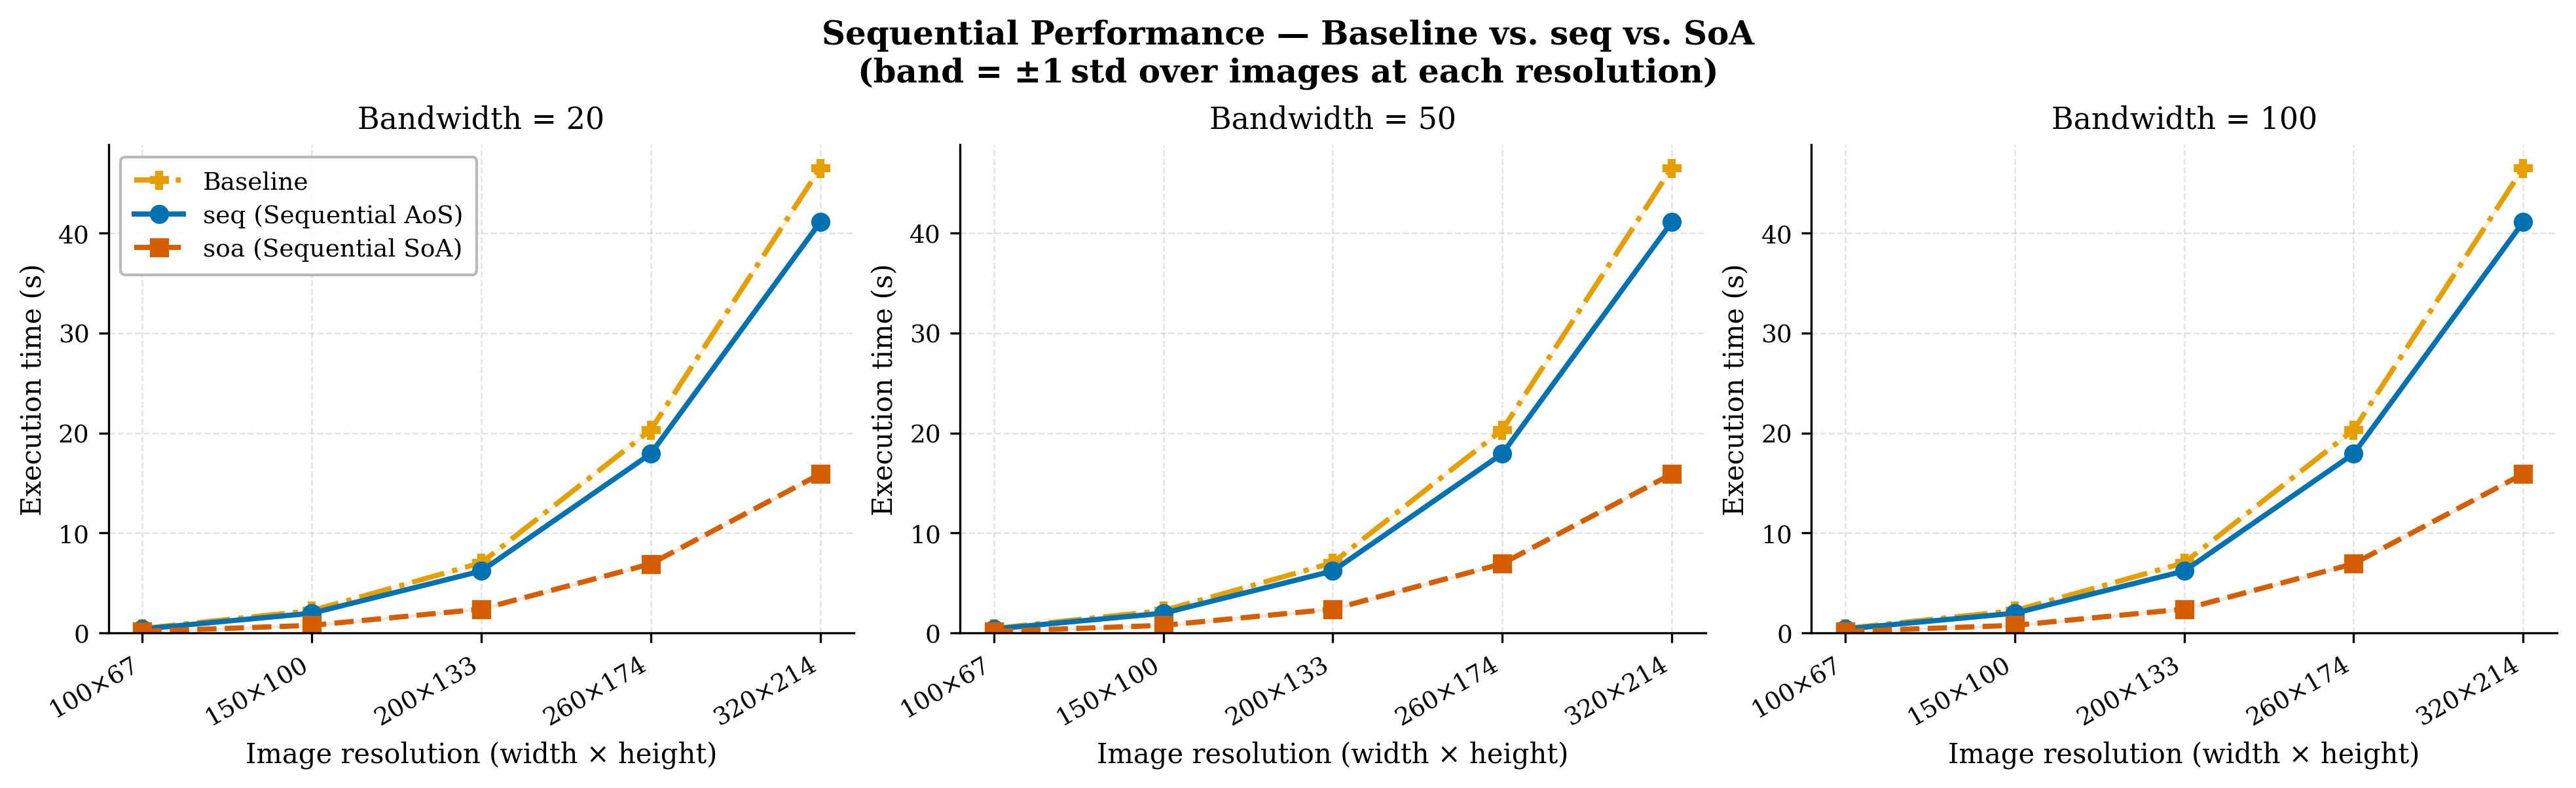
\includegraphics[width=1\linewidth]{images/fig_seq_comparison.png}
  
  \caption{Structure of Arrays (SoA) exhibits superior cache locality and throughput compared to Array of Structures (AoS) and Baseline, achieving a ~2.8× reduction in execution latency at higher resolutions. The invariance of performance across bandwidth settings (20–100) suggests a compute-bound or cache-latency-bound bottleneck rather than a memory bandwidth limitation. Shaded regions denote $\pm 1$ standard deviation across diverse image sets.}
    \label{fig:aos_soa}

    \end{center}
\end{figure*}
\subsection{Parallelization with OpenMP}


\subsection{CUDA}
\section{Conclusion}

\begin{figure*}
\begin{center}
\fbox{\rule{0pt}{2in} \rule{.9\linewidth}{0pt}}
\end{center}
   \caption{Example of a short caption, which should be centered.}
\label{fig:short}
\end{figure*}


\begin{figure*}[t]
    \centering
    % First Subfigure
    \begin{subfigure}[b]{0.32\textwidth}
        \centering
        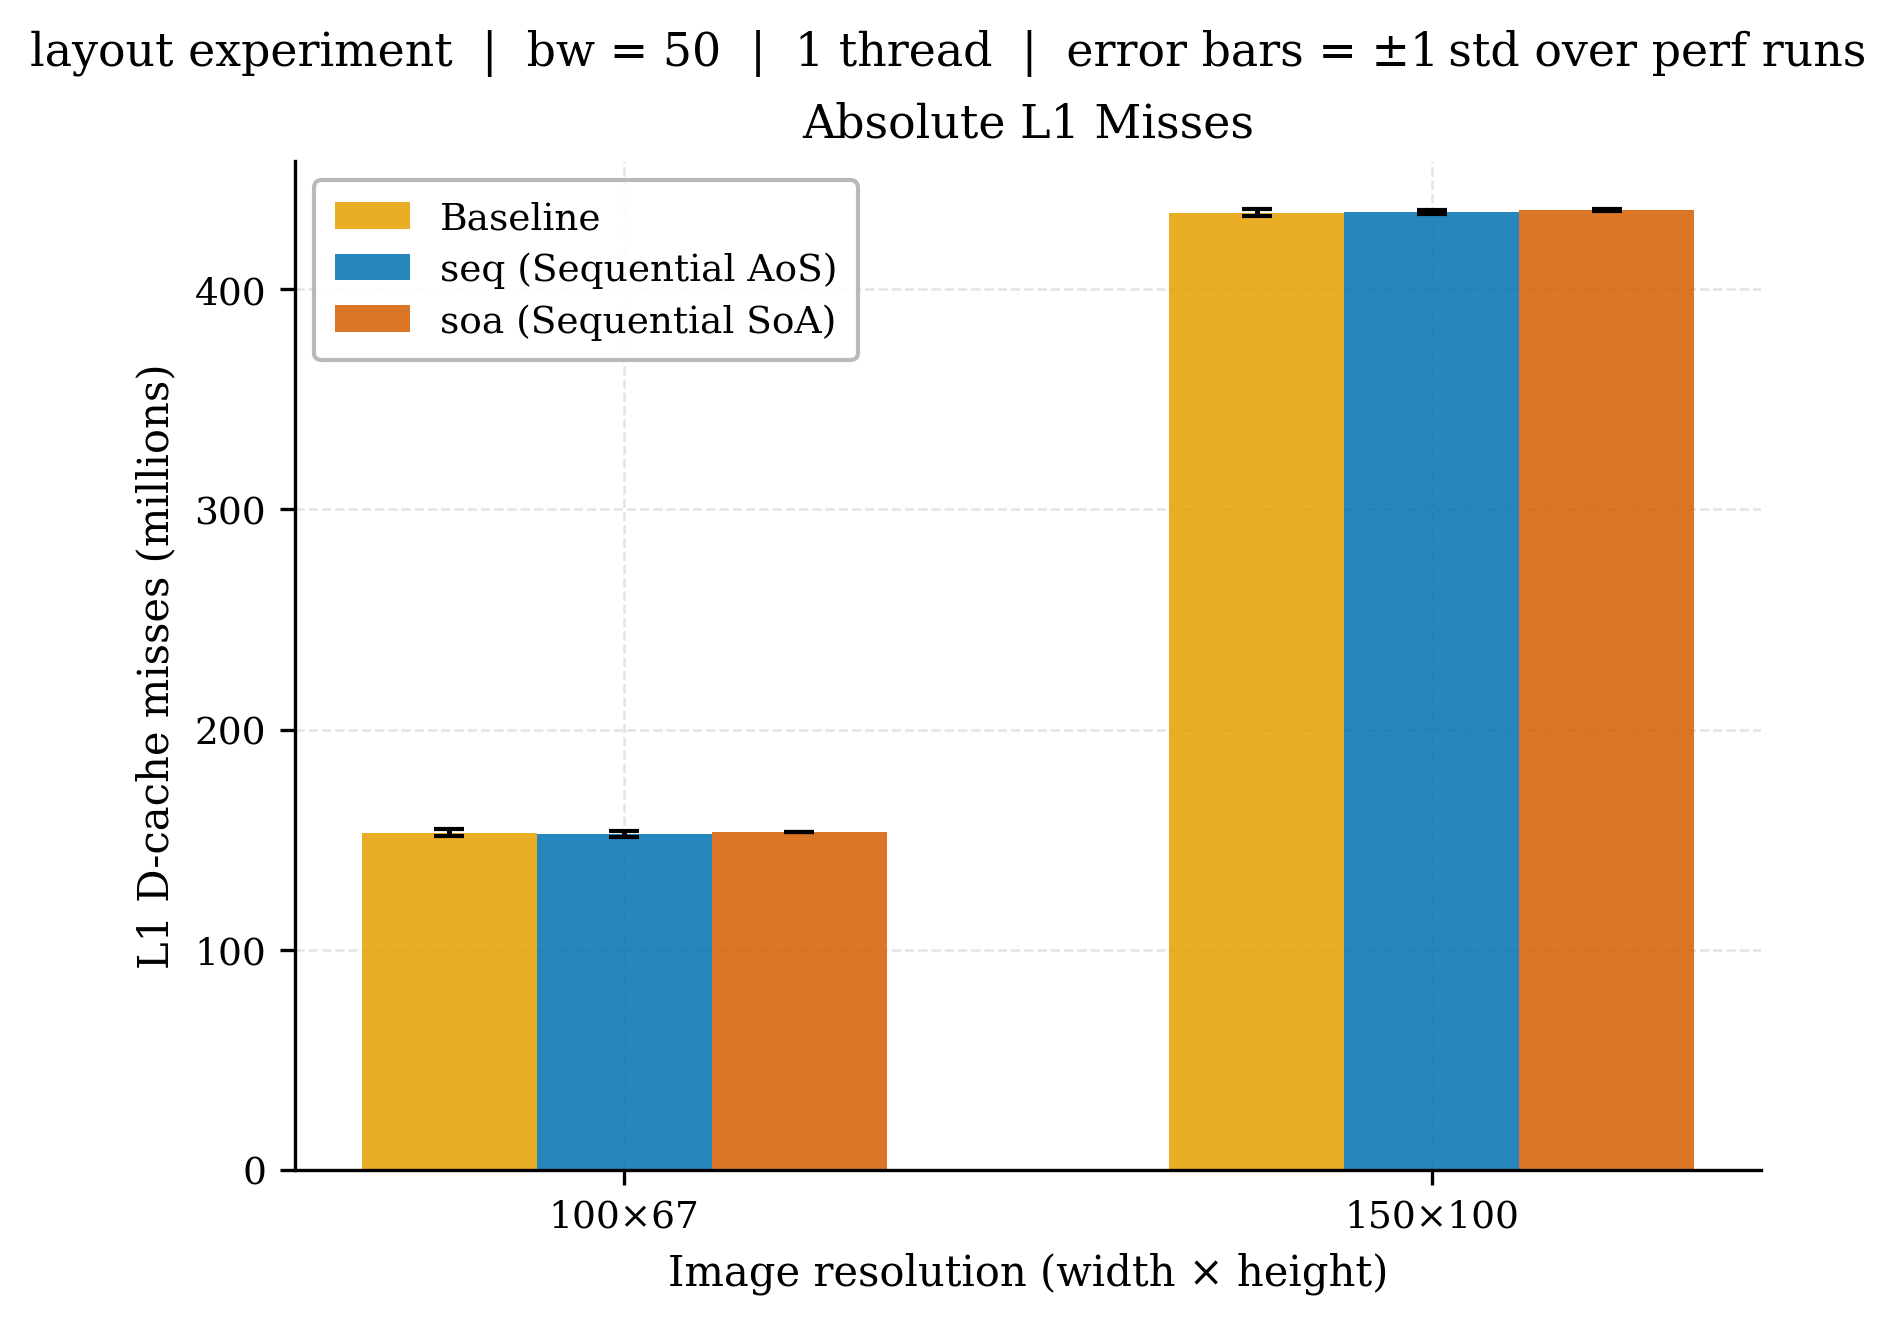
\includegraphics[width=\linewidth]{images/fig_profile_l1_miss_count.png}
        \caption{L1 Miss Count}
        \label{fig:profile_l1_miss_count}
    \end{subfigure}
    \hfill
    % Second Subfigure
    \begin{subfigure}[b]{0.32\textwidth}
        \centering
        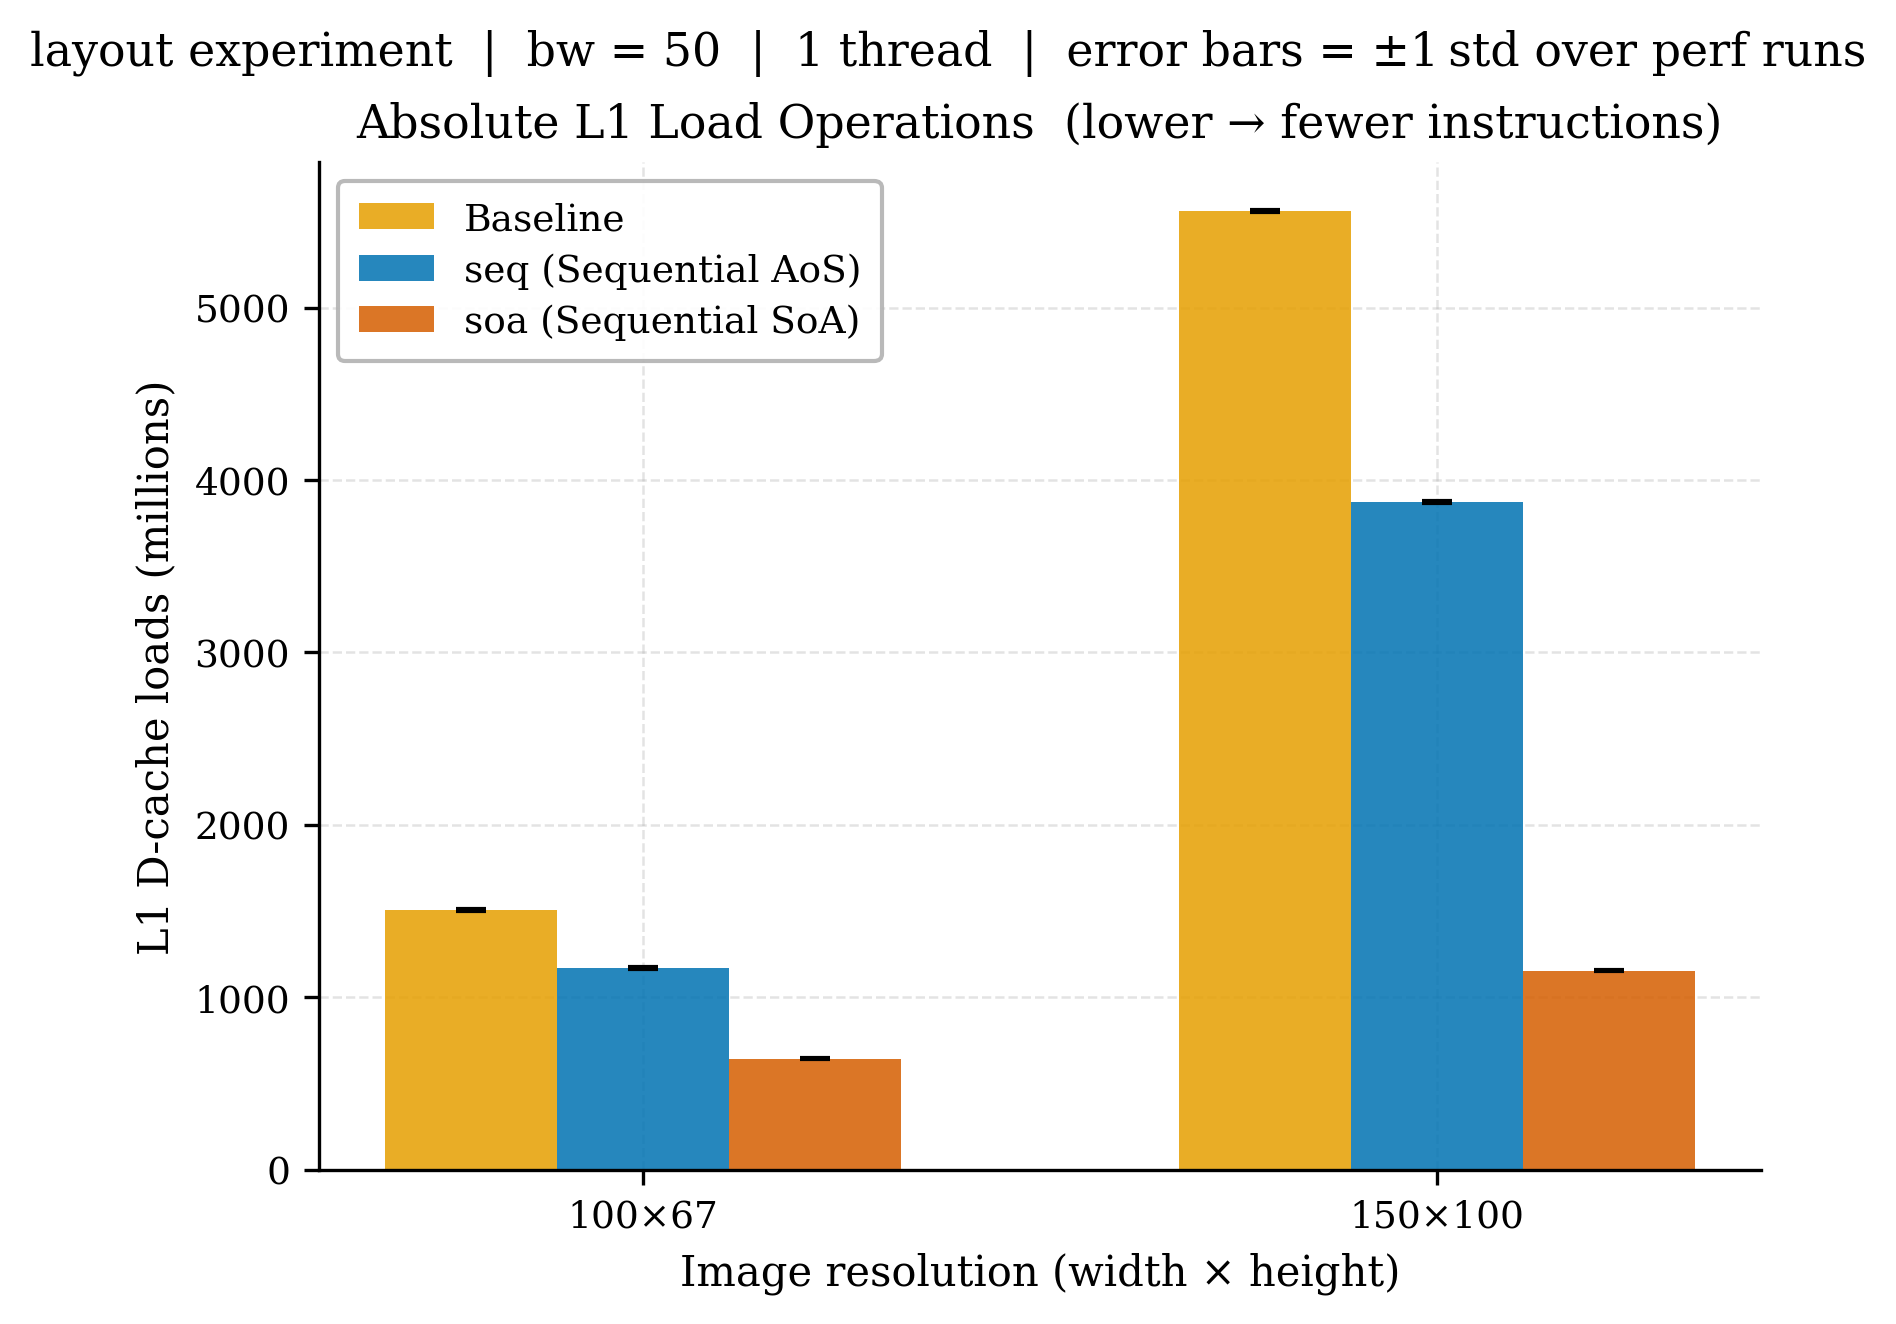
\includegraphics[width=\linewidth]{images/fig_profile_l1_loads.png}
        \caption{L1 Loads}
        \label{fig:profile_l1_loads}
    \end{subfigure}
    \hfill
    % Third Subfigure
    \begin{subfigure}[b]{0.32\textwidth}
        \centering
        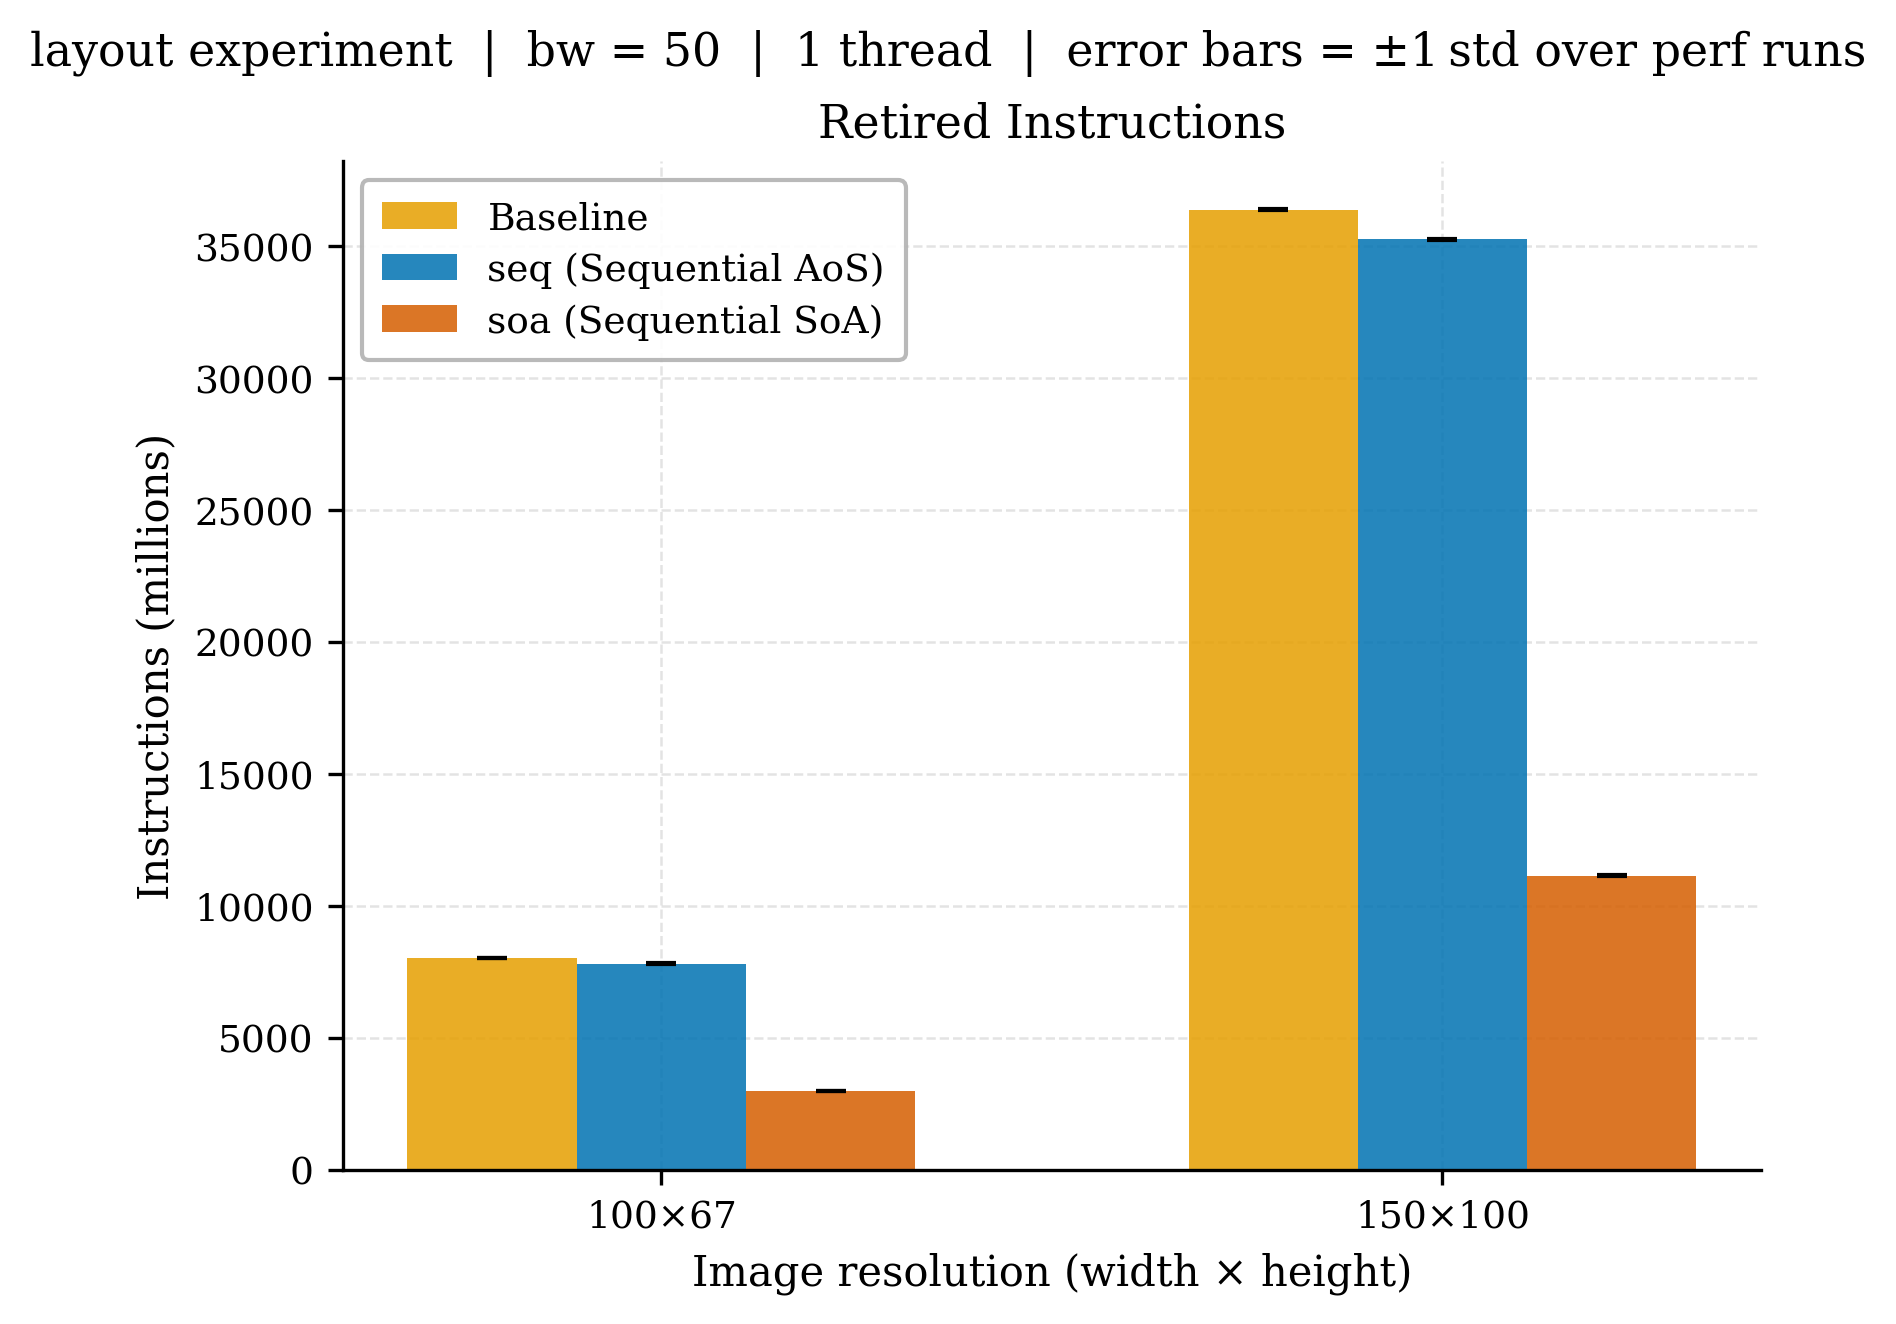
\includegraphics[width=\linewidth]{images/fig_profile_instructions.png}
        \caption{Instructions}
        \label{fig:profile_instructions}
    \end{subfigure}
    
    % Main Combined Caption
    \caption{Comprehensive profile metrics including L1 cache misses, total loads, and instruction counts.}
    \label{fig:profile_combined}
\end{figure*}



%------------------------------------------------------------------------
{\small
\bibliographystyle{ieee}
\bibliography{egbib}
}


\section{Appendix}\label{sec:appendix}
\subsection{The Baseline algorithm}\label{subsec:baseline}
\begin{lstlisting}[language=C++, caption={Sequential brute-force Mean Shift function}]
meanShiftResult meanShiftBaseline(STBImage& image, float bandwidth,
                                  int max_iter, float tol, bool show_pbar, KernelFn kernel) {
    using clock = std::chrono::steady_clock;

    if(!kernel) kernel = makeKernel("flat");

    const int width = image.width;
    const int n_pixels = image.width * image.height;
    uint8_t* raw = image.rgb_image;

    // Load raw uint8_t* into float working buffer
    std::vector<float> current(n_pixels * 3);
    for(int i = 0; i < n_pixels * 3; ++i)
        current[i] = static_cast<float>(raw[i]);

    const float bandwidth_sq = bandwidth * bandwidth;

    double total_shift_ms = 0.0;
    int iter = 0;
    std::vector<IterationInfo> iter_details;

    for(; iter < max_iter; ++iter) {
        std::vector<float> next(n_pixels * 3);
        float max_change = 0.0f;

        auto t_shift_start = clock::now();

        for(int i = 0; i < n_pixels; ++i) {
            float sum_r = 0.0f, sum_g = 0.0f, sum_b = 0.0f;
            float weight_sum = 0.0f;

            for(int j = 0; j < n_pixels; ++j) {
                float w = kernel(squaredDistanceBaseline(current, i, j, width), bandwidth_sq);
                if(w > 0.0f) {
                    sum_r += w * current[j * 3 + 0];
                    sum_g += w * current[j * 3 + 1];
                    sum_b += w * current[j * 3 + 2];
                    weight_sum += w;
                }
            }

            float change = 0.0f;
            if(weight_sum > 0.0f) {
                float new_r = sum_r / weight_sum;
                float new_g = sum_g / weight_sum;
                float new_b = sum_b / weight_sum;
                change = std::max({std::abs(new_r - current[i * 3 + 0]),
                                   std::abs(new_g - current[i * 3 + 1]),
                                   std::abs(new_b - current[i * 3 + 2])});
                next[i * 3 + 0] = new_r;
                next[i * 3 + 1] = new_g;
                next[i * 3 + 2] = new_b;
            } else {
                next[i * 3 + 0] = current[i * 3 + 0];
                next[i * 3 + 1] = current[i * 3 + 1];
                next[i * 3 + 2] = current[i * 3 + 2];
            }

            if(change > max_change)
                max_change = change;
        }

        auto t_shift_end = clock::now();
        double iter_ms = std::chrono::duration<double, std::milli>(t_shift_end - t_shift_start).count();
        total_shift_ms += iter_ms;
        iter_details.push_back({iter + 1, iter_ms, max_change});

        current.swap(next);

        if(show_pbar)
            printProgressBar(iter + 1, max_iter, max_change);

        if(max_change <= tol)
            break;
    }

    if(show_pbar)
        std::fprintf(stderr, "\n");

    // Write results back to raw uint8_t* buffer
    for(int i = 0; i < n_pixels * 3; ++i) {
        float val = std::max(0.0f, std::min(current[i], 255.0f));
        raw[i] = static_cast<uint8_t>(std::round(val));
    }

    return MeanShiftResult{static_cast<int>(iter_details.size()), total_shift_ms, iter_details};
}
\end{lstlisting}

\subsection{The \textit{seq} algorithm}\label{subsec:seq_code}
\begin{lstlisting}[language=C++, caption={Sequential Mean Shift function (seq)}]
MeanShiftResult meanShift(std::vector<uint8_t>& data, int width, float bandwidth,
                          int max_iter, float tol, bool show_pbar, KernelFn kernel) {
    using clock = std::chrono::steady_clock;

    if(!kernel) kernel = makeKernel("flat");

    auto t_conv_start = clock::now();
    std::vector<Pixel> current;
    toPixels(data, current, width);
    auto t_conv_end = clock::now();
    double convert_ms = std::chrono::duration<double, std::milli>(t_conv_end - t_conv_start).count();

    const float bandwidth_sq = bandwidth * bandwidth;
    const int n_pixels = static_cast<int>(current.size());

    double total_shift_ms = 0.0;
    int iter = 0;
    std::vector<IterationInfo> iter_details;

    // Hoist next outside the iteration loop - allocate once, reuse every iteration.
    std::vector<Pixel> next(n_pixels);

    for(; iter < max_iter; ++iter) {
        float max_change = 0.0f;

        auto t_shift_start = clock::now();

        for(int i = 0; i < n_pixels; ++i) {
            const Pixel& src = current[i];
            float sum_r = 0.0f, sum_g = 0.0f, sum_b = 0.0f;
            float weight_sum = 0.0f;

            for(int j = 0; j < n_pixels; ++j) {
                float w = kernel(squaredDistance(src, current[j]), bandwidth_sq);
                if(w > 0.0f) {
                    sum_r += w * current[j].r;
                    sum_g += w * current[j].g;
                    sum_b += w * current[j].b;
                    weight_sum += w;
                }
            }

            float change = 0.0f;
            if(weight_sum > 0.0f) {
                float new_r = sum_r / weight_sum;
                float new_g = sum_g / weight_sum;
                float new_b = sum_b / weight_sum;
                change = std::max({std::abs(new_r - src.r),
                                   std::abs(new_g - src.g),
                                   std::abs(new_b - src.b)});
                next[i] = {new_r, new_g, new_b, src.x, src.y};
            } else {
                next[i] = src;
            }

            if(change > max_change)
                max_change = change;
        }

        auto t_shift_end = clock::now();
        double iter_ms = std::chrono::duration<double, std::milli>(t_shift_end - t_shift_start).count();
        total_shift_ms += iter_ms;
        iter_details.push_back({iter + 1, iter_ms, max_change});

        current.swap(next);

        if(show_pbar)
            printProgressBar(iter + 1, max_iter, max_change);

        if(max_change <= tol)
            break;
    }

    if(show_pbar)
        std::fprintf(stderr, "\n");

    auto t_conv_out_start = clock::now();
    fromPixels(current, data);
    auto t_conv_out_end = clock::now();
    convert_ms += std::chrono::duration<double, std::milli>(t_conv_out_end - t_conv_out_start).count();

    return MeanShiftResult{static_cast<int>(iter_details.size()), total_shift_ms, convert_ms, iter_details};
}

\end{lstlisting}

\subsection{The \textit{soa} algorithm}\label{subsec:soa_code}
\begin{lstlisting}[language=C++, caption={SoA brute-force Mean Shift function}]
MeanShiftResult meanShiftSoA(std::vector<uint8_t>& data, int width, float bandwidth,
                             int max_iter, float tol, bool show_pbar, KernelFn kernel) {
    using clock = std::chrono::steady_clock;

    if(!kernel) kernel = makeKernel("flat");

    auto t_conv_start = clock::now();
    std::vector<float> current;
    convertToFloat(data, current);

    ImageSoA soa;
    convertToFloatSoA(current, soa, width);
    auto t_conv_end = clock::now();
    double convert_ms = std::chrono::duration<double, std::milli>(t_conv_end - t_conv_start).count();

    const float bandwidth_sq = bandwidth * bandwidth;
    int n_pixels = soa.n;

    double total_shift_ms = 0.0;
    int iter = 0;
    std::vector<IterationInfo> iter_details;

    // Hoist next buffers outside the iteration loop - allocate once, reuse every iteration.
    std::vector<float> next_r(n_pixels);
    std::vector<float> next_g(n_pixels);
    std::vector<float> next_b(n_pixels);

    for(; iter < max_iter; ++iter) {
        float max_change = 0.0f;

        auto t_shift_start = clock::now();

        for(int i = 0; i < n_pixels; ++i) {
            NeighborAccumulator acc;

            for(int j = 0; j < n_pixels; ++j) {
                float w = kernel(squaredDistanceSoA(soa, i, j), bandwidth_sq);
                if(w > 0.0f) {
                    acc.sum_r += w * soa.r[j];
                    acc.sum_g += w * soa.g[j];
                    acc.sum_b += w * soa.b[j];
                    acc.weight_sum += w;
                }
            }

            float change = 0.0f;
            if(acc.weight_sum > 0.0f) {
                float new_r = acc.sum_r / acc.weight_sum;
                float new_g = acc.sum_g / acc.weight_sum;
                float new_b = acc.sum_b / acc.weight_sum;

                float dr = new_r - soa.r[i];
                float dg = new_g - soa.g[i];
                float db = new_b - soa.b[i];

                change = std::max({std::abs(dr), std::abs(dg), std::abs(db)});

                next_r[i] = new_r;
                next_g[i] = new_g;
                next_b[i] = new_b;
            } else {
                next_r[i] = soa.r[i];
                next_g[i] = soa.g[i];
                next_b[i] = soa.b[i];
            }

            if(change > max_change)
                max_change = change;
        }

        auto t_shift_end = clock::now();
        double iter_ms = std::chrono::duration<double, std::milli>(t_shift_end - t_shift_start).count();
        total_shift_ms += iter_ms;
        iter_details.push_back({iter + 1, iter_ms, max_change});

        soa.r.swap(next_r);
        soa.g.swap(next_g);
        soa.b.swap(next_b);

        if(show_pbar)
            printProgressBar(iter + 1, max_iter, max_change);

        if(max_change <= tol)
            break;
    }

    if(show_pbar)
        std::fprintf(stderr, "\n");

    auto t_conv_out_start = clock::now();
    convertFromFloatSoA(soa, current);
    convertFromFloat(current, data);
    auto t_conv_out_end = clock::now();
    convert_ms += std::chrono::duration<double, std::milli>(t_conv_out_end - t_conv_out_start).count();

    return MeanShiftResult{static_cast<int>(iter_details.size()), total_shift_ms, convert_ms, iter_details};
}
\end{lstlisting}

\subsection{The \textit{omp} algorithm}\label{subsec:omp_code}
\begin{lstlisting}[language=C++, caption={Parallel brute-force Mean Shift function}]
MeanShiftResult meanShiftOMP(std::vector<uint8_t>& data, int width, float bandwidth,
                             int max_iter, float tol, bool show_pbar, KernelFn kernel) {
    using clock = std::chrono::steady_clock;

    if(!kernel) kernel = makeKernel("flat");

    auto t_conv_start = clock::now();
    std::vector<Pixel> current;
    toPixelsOMP(data, current, width);
    auto t_conv_end = clock::now();
    double convert_ms = std::chrono::duration<double, std::milli>(t_conv_end - t_conv_start).count();

    const float bandwidth_sq = bandwidth * bandwidth;
    const int n_pixels = static_cast<int>(current.size());

    // Hoist next outside the iteration loop - allocate once, reuse every iteration.
    std::vector<Pixel> next(n_pixels);

    double total_shift_ms = 0.0;
    int iter = 0;
    std::vector<IterationInfo> iter_details;

    for(; iter < max_iter; ++iter) {
        float max_change = 0.0f;

        auto t_shift_start = clock::now();

        #pragma omp parallel for schedule(static) reduction(max:max_change)
        for(int i = 0; i < n_pixels; ++i) {
            const Pixel& src = current[i];
            float sum_r = 0.0f, sum_g = 0.0f, sum_b = 0.0f;
            float weight_sum = 0.0f;

            for(int j = 0; j < n_pixels; ++j) {
                float w = kernel(squaredDistanceOMP(src, current[j]), bandwidth_sq);
                if(w > 0.0f) {
                    sum_r += w * current[j].r;
                    sum_g += w * current[j].g;
                    sum_b += w * current[j].b;
                    weight_sum += w;
                }
            }

            float change = 0.0f;
            if(weight_sum > 0.0f) {
                float new_r = sum_r / weight_sum;
                float new_g = sum_g / weight_sum;
                float new_b = sum_b / weight_sum;
                change = std::max({std::abs(new_r - src.r),
                                   std::abs(new_g - src.g),
                                   std::abs(new_b - src.b)});
                next[i] = {new_r, new_g, new_b, src.x, src.y};
            } else {
                next[i] = src;
            }

            max_change = std::max(max_change, change);
        }

        auto t_shift_end = clock::now();
        double iter_ms = std::chrono::duration<double, std::milli>(t_shift_end - t_shift_start).count();
        total_shift_ms += iter_ms;
        iter_details.push_back({iter + 1, iter_ms, max_change});

        current.swap(next);

        if(show_pbar)
            printProgressBar(iter + 1, max_iter, max_change);

        if(max_change <= tol)
            break;
    }

    if(show_pbar)
        std::fprintf(stderr, "\n");

    auto t_conv_out_start = clock::now();
    fromPixelsOMP(current, data);
    auto t_conv_out_end = clock::now();
    convert_ms += std::chrono::duration<double, std::milli>(t_conv_out_end - t_conv_out_start).count();

    return MeanShiftResult{static_cast<int>(iter_details.size()), total_shift_ms, convert_ms, iter_details};
}
\end{lstlisting}

\subsection{The \textit{omp\_soa} algorithm}\label{subsec:omp_soa_code}
\begin{lstlisting}[language=C++, caption={Parallel (SoA) brute-force Mean Shift function}]
MeanShiftResult meanShiftSoAOMP(std::vector<uint8_t>& data, int width, float bandwidth,
                                int max_iter, float tol, bool show_pbar, KernelFn kernel) {
    using clock = std::chrono::steady_clock;

    if(!kernel) kernel = makeKernel("flat");

    auto t_conv_start = clock::now();
    std::vector<float> current;
    convertToFloat(data, current);

    ImageSoA soa;
    convertToFloatSoA(current, soa, width);
    auto t_conv_end = clock::now();
    double convert_ms = std::chrono::duration<double, std::milli>(t_conv_end - t_conv_start).count();

    const float bandwidth_sq = bandwidth * bandwidth;
    int n_pixels = soa.n;

    // Hoist next buffers outside the iteration loop - allocate once, reuse every iteration.
    std::vector<float> next_r(n_pixels);
    std::vector<float> next_g(n_pixels);
    std::vector<float> next_b(n_pixels);

    double total_shift_ms = 0.0;
    int iter = 0;
    std::vector<IterationInfo> iter_details;

    for(; iter < max_iter; ++iter) {
        float max_change = 0.0f;

        auto t_shift_start = clock::now();

        #pragma omp parallel for schedule(static) reduction(max:max_change)
        for(int i = 0; i < n_pixels; ++i) {
            NeighborAccumulator acc;

            for(int j = 0; j < n_pixels; ++j) {
                float w = kernel(squaredDistanceSoA(soa, i, j), bandwidth_sq);
                if(w > 0.0f) {
                    acc.sum_r += w * soa.r[j];
                    acc.sum_g += w * soa.g[j];
                    acc.sum_b += w * soa.b[j];
                    acc.weight_sum += w;
                }
            }

            float change = 0.0f;
            if(acc.weight_sum > 0.0f) {
                float new_r = acc.sum_r / acc.weight_sum;
                float new_g = acc.sum_g / acc.weight_sum;
                float new_b = acc.sum_b / acc.weight_sum;

                float dr = new_r - soa.r[i];
                float dg = new_g - soa.g[i];
                float db = new_b - soa.b[i];

                change = std::max({std::abs(dr), std::abs(dg), std::abs(db)});

                next_r[i] = new_r;
                next_g[i] = new_g;
                next_b[i] = new_b;
            } else {
                next_r[i] = soa.r[i];
                next_g[i] = soa.g[i];
                next_b[i] = soa.b[i];
            }

            if(change > max_change)
                max_change = change;
        }

        auto t_shift_end = clock::now();
        double iter_ms = std::chrono::duration<double, std::milli>(t_shift_end - t_shift_start).count();
        total_shift_ms += iter_ms;
        iter_details.push_back({iter + 1, iter_ms, max_change});

        soa.r.swap(next_r);
        soa.g.swap(next_g);
        soa.b.swap(next_b);

        if(show_pbar)
            printProgressBar(iter + 1, max_iter, max_change);

        if(max_change <= tol)
            break;
    }

    if(show_pbar)
        std::fprintf(stderr, "\n");

    auto t_conv_out_start = clock::now();
    convertFromFloatSoA(soa, current);
    convertFromFloat(current, data);
    auto t_conv_out_end = clock::now();
    convert_ms += std::chrono::duration<double, std::milli>(t_conv_out_end - t_conv_out_start).count();

    return MeanShiftResult{static_cast<int>(iter_details.size()), total_shift_ms, convert_ms, iter_details};
}

\end{lstlisting}

\begin{lstlisting}[language=C++, caption={Structure of Arrays (SoA) representation and weighted neighbor accumulator for intermediate calculations}, label={code:soa_impl_with_neigh_acc}]
// SoA pixel representation - separate channels for better parallelism
struct ImageSoA {
    std::vector<float> r;
    std::vector<float> g;
    std::vector<float> b;
    std::vector<float> x;  // spatial column coordinate (fixed)
    std::vector<float> y;  // spatial row coordinate (fixed)
    int n;
};

// SoA neighbor accumulator - uses float weight_sum to support weighted kernels
struct NeighborAccumulator {
    float sum_r = 0.0f;
    float sum_g = 0.0f;
    float sum_b = 0.0f;
    float weight_sum = 0.0f;
};
\end{lstlisting}

\begin{figure*}

\begin{center}
    \begin{subfigure}[c]{\textwidth}
    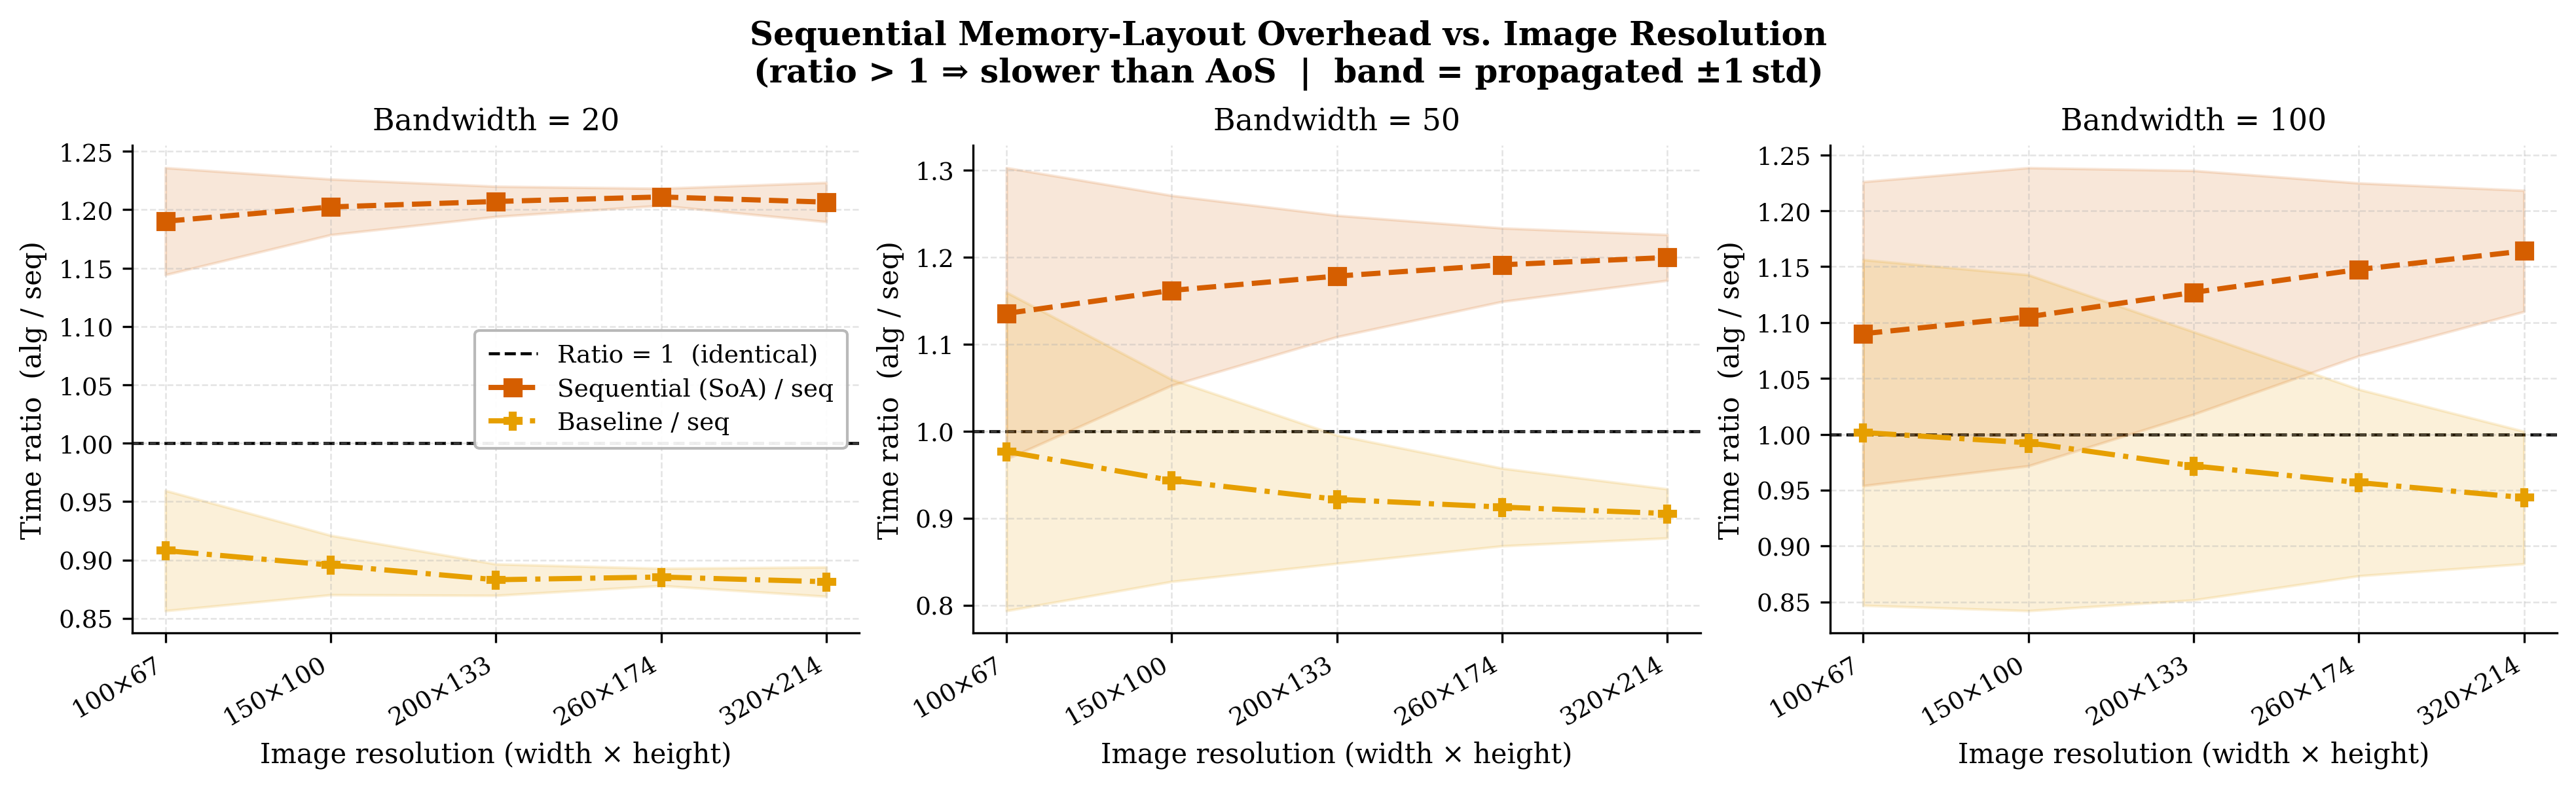
\includegraphics[width=\linewidth]{images/fig_seq_layout_overhead_problem.png}
    \label{subfig:mem_layout}
    \caption{}
    \end{subfigure}
    \begin{subfigure}[c]{\textwidth}
    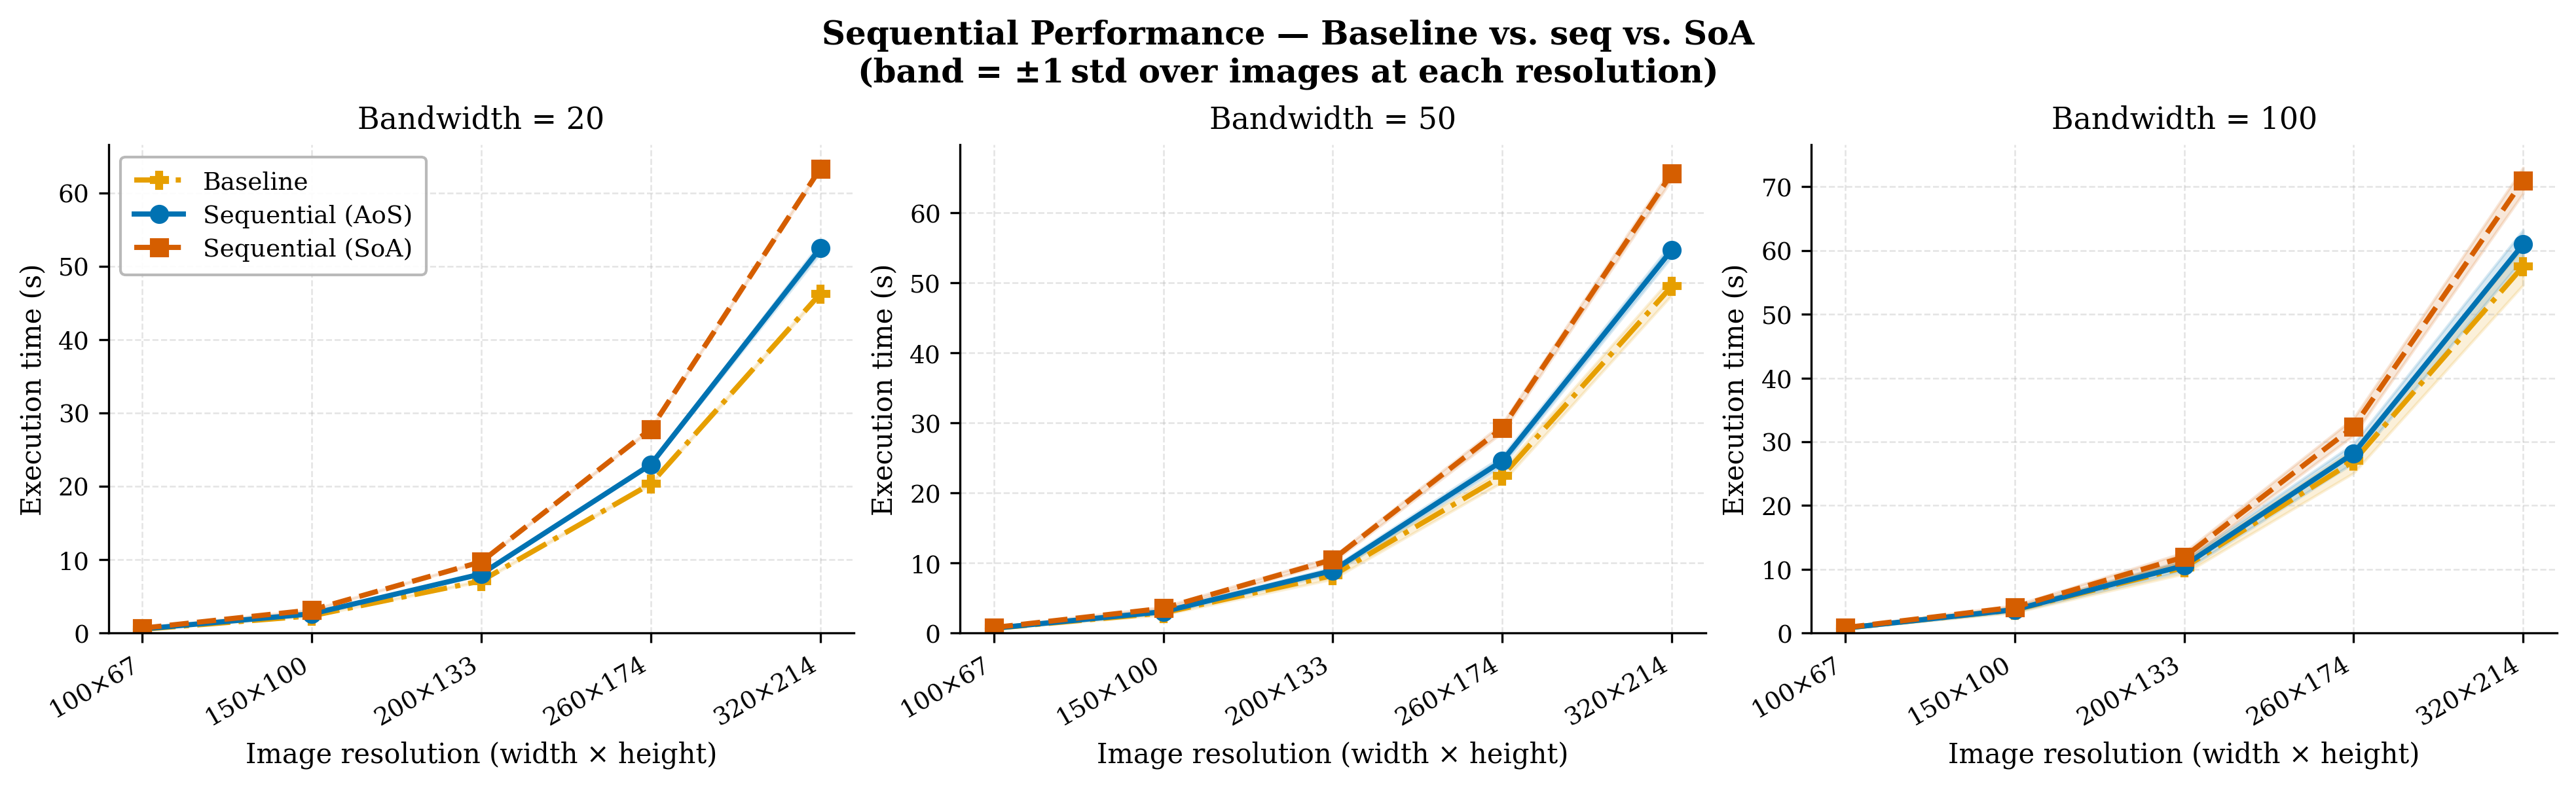
\includegraphics[width=\linewidth]{images/fig_seq_comparison_problem.png}
    \label{subfig:seq_comp}
    \caption{}
  
    \end{subfigure}
    \begin{subfigure}[c]{\textwidth}
    
    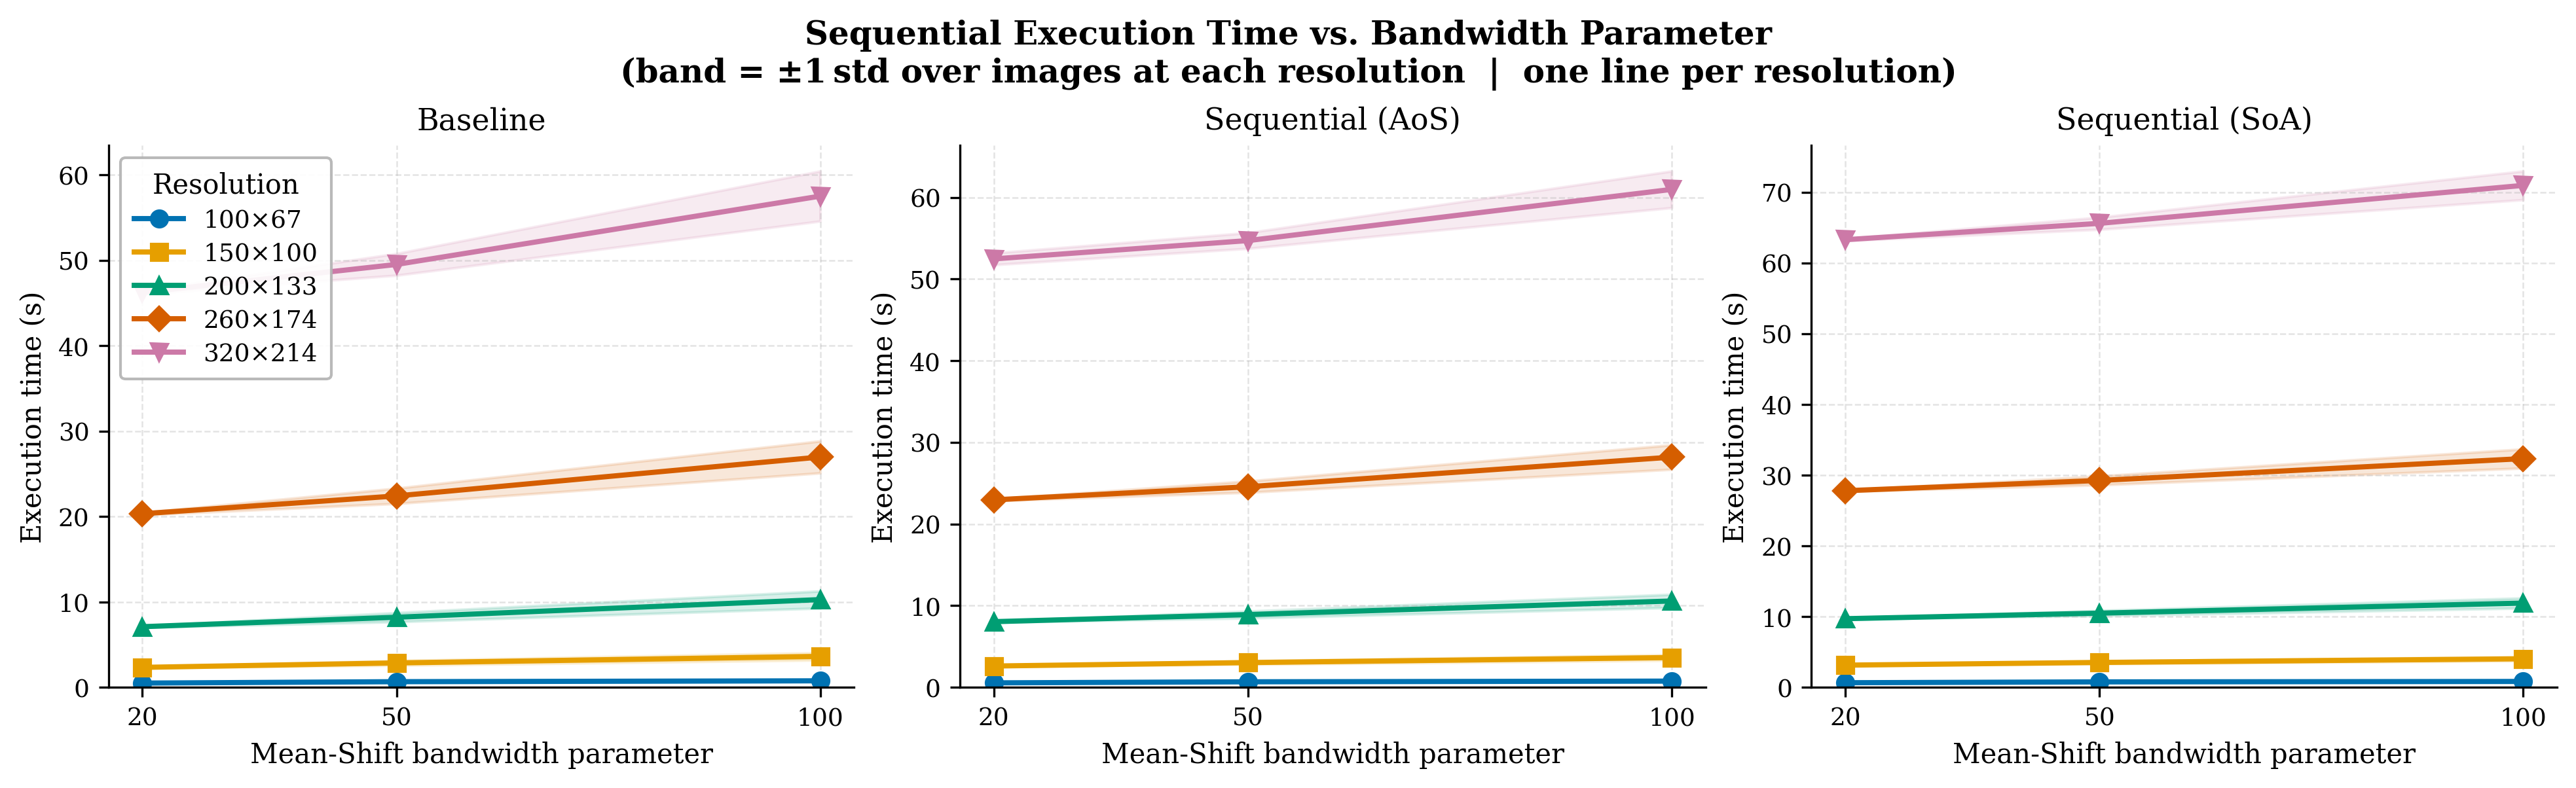
\includegraphics[width=\linewidth]{fig_seq_bw_comparison_problem.png}
    \label{subfig:seq_bw_comp}
    \caption{}
    \end{subfigure}
\caption{Sequential performance profiling of Mean Shift variants utilizing a dynamically swappable kernel on the AMD Ryzen 9900X. The abstraction overhead of this kernel design fundamentally inhibits compiler auto-vectorization. The resulting absence of SIMD acceleration dictates the anomalous performance characteristics observed across all three subfigures. 
\textbf{(a)} Memory layout overhead. The naive Baseline unexpectedly outperforms both pre-computed AoS and SoA layouts. Without SIMD registers to rapidly consume contiguous data, the memory-bound optimizations of SoA introduce detrimental scalar load latency. 
\textbf{(b)} Execution latency scaling. The Baseline maintains superior performance across spatial resolutions. In a purely scalar execution regime, the overhead of fetching disparate pre-computed coordinates from the L1 cache exceeds the latency of the Baseline's on-the-fly arithmetic recomputation. 
\textbf{(c)} Bandwidth dependency. Expanding the spatial bandwidth introduces a distinct latency penalty. Lacking SIMD units to efficiently parallelize the $\mathcal{O}(N^2)$ neighbor evaluations, the pipeline becomes saturated by compute-bound scalar operations, exposing the direct arithmetic cost of the expanded search volume.}
    \label{fig:sequential_performance_analysis}
    \label{fig:kernel_problem}

    \end{center}
\end{figure*}

\end{document}





%%% Some comments:
Parallelize outer for i in 0..n — each pixel's new position is independent (Jacobi). This is what we implement.
The inner for j sum that determines which pixels fall within the bandwidth. Could be parallelized with a thread-local reduction, but less efficient than outer loop. Documented as a considered alternative.
Post-processing: label pixels that converged to the same mode as the same cluster. Our code doesn't have an explicit mode detection step (colors after convergence serve as cluster labels implicitly), but this step would be fully parallelizable if added. Documented.
%%% 

\subsection{Data Structures}
A central challenge in implementing the 5D Mean Shift algorithm is managing memory access patterns within the $O(N^2)$ inner loop. We evaluate two primary data layouts for image storage: \textbf{Array of Structures (AoS)} and \textbf{Structure of Arrays (SoA)}. These layouts significantly impact cache line utilization and the compiler’s ability to generate SIMD instructions. The initial image data provided by the \texttt{stb\_image} library is stored in a standard interleaved RGB buffer, which we then transform into our internal feature space representation.

\subsubsection{Baseline Implementation (AoS)}
The baseline implementation utilizes an implicit \textbf{Array of Structures (AoS)} layout to represent the image data. In this configuration, the color channels are interleaved and stored contiguously in memory as $[R_0, G_0, B_0, R_1, G_1, B_1, \dots]$, as shown in Listing~\ref{code:aos_impl}. 

To minimize the memory footprint of this baseline version, spatial coordinates $(x, y)$ are not explicitly stored in the feature vector. Instead, they are derived dynamically from the pixel index $j$ and the image width during each iteration of the inner loop (Listing~\ref{code:aos_spatial}). 



While this approach minimizes memory consumption, it introduces a significant computational bottleneck. Integer division (\texttt{/}) and modulo (\texttt{\%}) are high-latency instructions; performing these operations $N^2$ times per iteration makes the inner loop heavily \textbf{compute-bound}. Profiling indicated that the CPU cycles spent on coordinate calculation significantly outweighed the distance math itself. 

To mitigate this, we transitioned to a strategy where spatial coordinates are pre-computed and stored alongside color values. This adjustment trades a minor increase in memory usage for a substantial reduction in per-iteration execution time, effectively shifting the bottleneck from the ALU to the memory subsystem. This transition laid the groundwork for the \textbf{Structure of Arrays (SoA)} optimization discussed in the following section.


\subsubsection{Baseline Implementation (AoS)}
The baseline implementation utilizes an interleaved memory layout, which we define as a \textit{logical} Array of Structures (AoS). Although the data is stored in a flat \texttt{std::vector<float>} rather than a formal C++ \texttt{struct}, the memory footprint is identical to an interleaved layout where all components of a single data element (the RGB channels) are stored contiguously. 

As defined in the Intel 64 and IA-32 Architectures Optimization Reference Manual \cite{intel_opt}, this layout is one where ``all the components of a single data element are stored contiguously in memory... often requiring de-interleaving for efficient SIMD processing.'' In our case, this contiguous grouping provides high spatial locality for single-pixel operations but introduces a stride-3 access pattern for individual color channels. This makes the loop difficult to auto-vectorize, as the CPU cannot load multiple values of the same channel into a SIMD register without expensive "gather" or "shuffle" instructions.



To further optimize this baseline, we explicitly pre-compute the spatial coordinates $(x, y)$ and store them, rather than calculating them on-the-fly using modulo and division. This ensures that the baseline represents a "best-case" sequential version that is bound by memory access patterns rather than artificial computational overhead.